\documentclass{article}

\usepackage{amsmath} % For mathematical symbols and environments
\usepackage{amssymb} % For additional mathematical symbols
\usepackage{tcolorbox}
\usepackage{pgfplots} % Add this line to import the pgfplots package

\newtcolorbox{esbox}{
    colback=blue!5!white,
    colframe=blue!75!black,
    fonttitle=\bfseries,
    title=Esempio
}

\title{Definizioni}
\author{Agostino Cesarano}
\date{January 2024}

\begin{document}

\maketitle
\setcounter{part}{3}
\part{Derivate}
Si chiama \textbf{rapporto incrementale} di $f(x)$ nel punto $x_0$ il rapporto
\begin{equation*}
    \frac{dy}{dx} = \frac{f(x_0 + h) - f(x_0)}{h}
\end{equation*}
\begin{figure}[h]
    \centering
    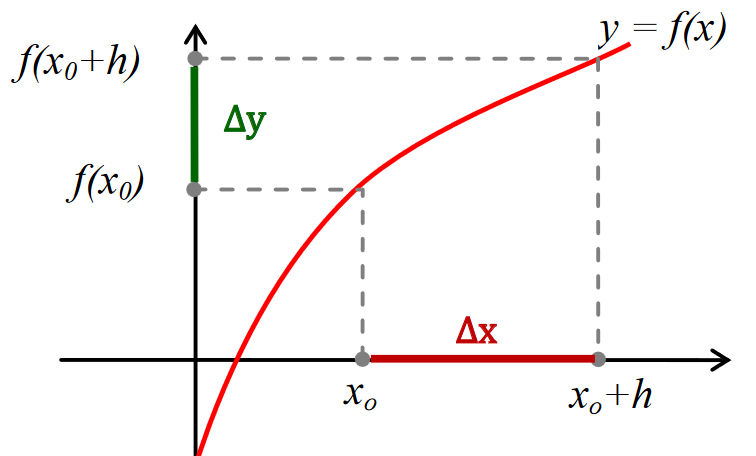
\includegraphics[width=0.5\textwidth]{rappincr.png}
    \caption{Rappresentazione grafica del rapporto incrementale}
\end{figure}
Sia $f(x)$ definita nell'intervallo aperto $(a,b)$ e sia $x \in (a,b)$. Si dice
che $f(x)$ è derivabile in $x$ se esiste il limite del rapporto incrementale
\begin{equation*}
    \lim_{h \to x_0} \frac{f(x+h)-f(x)}{h}
\end{equation*}
e si indica con $f'(x_0)$.\\
Sia $f(x)$ definita nell'intervallo aperto $(a,b)$ e sia $x \in (a,b)$. Si dice
che $f(x)$ è derivabile in $x$ se esiste il limite del rapporto incrementale.\\\\
Se una funzione è derivabile in un punto, allora è anche continua in quel punto.
\newpage
%Derivata sinistra e destra%
Si definisce derivata a sinistra di $f(x)$ nel punto $x_0$ il limite
\begin{equation*}
    \lim_{h \to 0^-} \frac{f(x_0+h)-f(x_0)}{h}
\end{equation*}
e si indica con $f'_-(x_0)$.
Si definisce derivata a destra di $f(x)$ nel punto $x_0$ il limite
\begin{equation*}
    \lim_{h \to 0^+} \frac{f(x_0+h)-f(x_0)}{h}
\end{equation*}
e si indica con $f'_+(x_0)$.\\\\
%Significato geometrico della derivata%
\textbf{Significato geometrico della derivata}\\
Sia $f(x)$ una funzione derivabile in $x_0$. Il valore della derivata
$f'(x_0)$ rappresenta la pendenza della retta tangente alla curva $y=f(x)$
nel punto $P(x_0,f(x_0))$.
\begin{figure}[h]
    \centering
    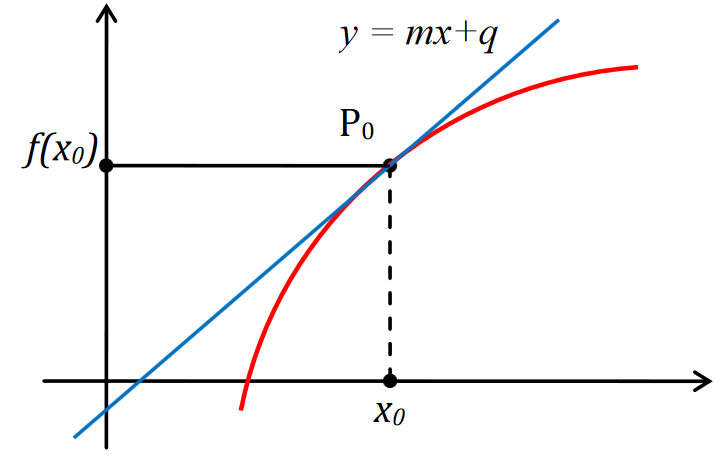
\includegraphics[width=0.5\textwidth]{derivgeom.png}
    \caption{Rappresentazione grafica del significato geometrico della derivata}
\end{figure}\\
%Operazioni con le derivate%
\textbf{Operazioni con le derivate}\\
Siano $f(x)$ e $g(x)$ due funzioni derivabili in $x_0$. Allora valgono le
seguenti proprietà:
\begin{itemize}
    \item $(f+g)'(x_0) = f'(x_0) + g'(x_0)$
    \item $(f-g)'(x_0) = f'(x_0) - g'(x_0)$
    \item $(f\cdot g)'(x_0) = f'(x_0)g(x_0) + f(x_0)g'(x_0)$
    \item $\left(\frac{f}{g}\right)'(x_0) = \frac{f'(x_0)g(x_0) -
                  f(x_0)g'(x_0)}{(g(x_0))^2}$
    \item $(f(g(x)))'(x_0) = f'(g(x_0))g'(x_0)$
\end{itemize}
Se $f(x)$ è una funzione continua e strettamente monotona in un intervallo $[a,b]$. Se $f(x)$ è derivabile in $x \in (a,b)$ e se $f'(x)\neq0$, allora $f^{-1}(x)$ è derivabile in $y = f(x)$ e la derivata vale
\begin{equation*}
    (f^{-1})'(x_0) = \frac{1}{f'(f^{-1}(x_0))}
\end{equation*}
\begin{esbox}
    $D\sqrt{y}=\frac{1}{D(x^2)}=\frac{1}{2x}=\frac{1}{2\sqrt{y}}$
\end{esbox}
\section*{Criterio di convessità}
Supponiamo che $f(x)$ sia derivabile in $[a,b]$ e che ammetta derivata seconda in $(a,b)$. Allora valgono le seguenti proprietà:
\begin{itemize}
    \item Se $f''(x)\geq0$ in $(a,b)$, allora $f(x)$ è convessa in $[a,b]$.
    \item Se $f''(x)\leq0$ in $(a,b)$, allora $f(x)$ è concava in $[a,b]$.
\end{itemize}
Per convessa si intende che la funzione è sempre sopra la sua tangente.
\begin{figure}[h]
    \centering
    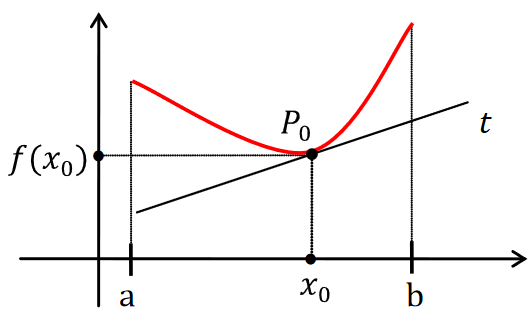
\includegraphics[width=0.5\textwidth]{convessa.png}
    \caption{Rappresentazione grafica di una funzione convessa}
\end{figure}\\
Per concava si intende che la funzione è sempre sotto la sua tangente.
\begin{figure}[h]
    \centering
    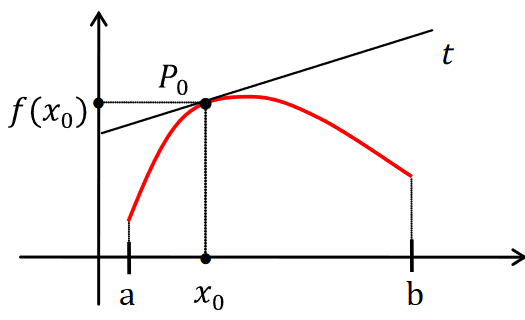
\includegraphics[width=0.5\textwidth]{concava.png}
    \caption{Rappresentazione grafica di una funzione concava}
\end{figure}\\
%punti di flesso%
\newpage
\textbf{Punti di flesso}\\
Sia $f(x)$ una funzione derivabile in $[a,b]$ e che ammetta derivata seconda in $(a,b)$. Se $f''(x)$ cambia segno in $x_0 \in (a,b)$, allora $P(x_0,f(x_0))$ è un punto di flesso.
\begin{figure}[h]
    \centering
    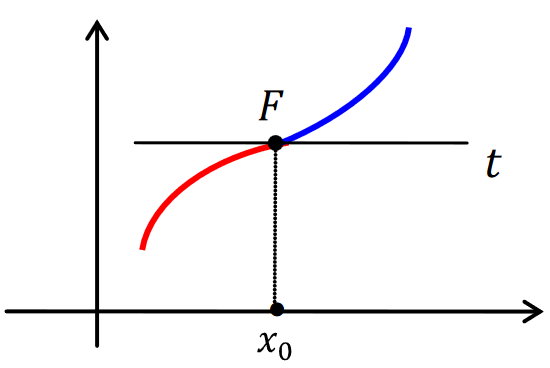
\includegraphics[width=0.4\textwidth]{flesso.png}
    \caption{Rappresentazione grafica di un punto di flesso}
\end{figure}\\
%Punti di non derivabilità%
\section*{Punti di non derivabilità}
I punti di non derivabilità sono quei punti che appartengono al dominio della funzione ma che non appartengono al dominio della derivata prima.\\
Questi punti si classificano in:
\begin{itemize}
\item \textbf{Punti angolosi} Un punto $x_0$ è angoloso se esiste il limite destro e sinistro della derivata prima ma non sono uguali.\\
\[
    \lim_{x \to x_0^+} f'(x) \neq \lim_{x \to x_0^-} f'(x)
\]
\begin{figure}[h]
    \centering
    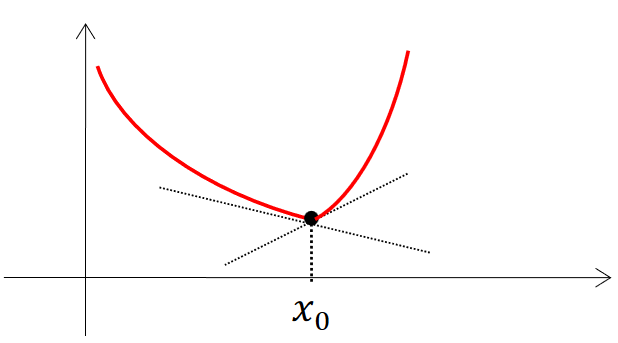
\includegraphics[width=0.4\textwidth]{angoloso.png}
    \caption{Rappresentazione grafica di un punto angoloso}
\end{figure}\\
Almeno una tra le due derivate destro e sinistro deve essere finita.
\newpage
\item \textbf{Punti di cuspide} Un punto $x_0$ è di cuspide se esiste il limite destro e sinistro della derivata prima non sono finiti e di segno opposto.\\
\[
    \lim_{x \to x_0^+} f'(x) = -\infty \quad \land \quad \lim_{x \to x_0^-} f'(x) = +\infty
\]
\begin{center}
    oppure
\end{center}
\[
    \lim_{x \to x_0^+} f'(x) = +\infty \quad \land \quad \lim_{x \to x_0^-} f'(x) = -\infty
\]
\begin{figure}[h]
\centering
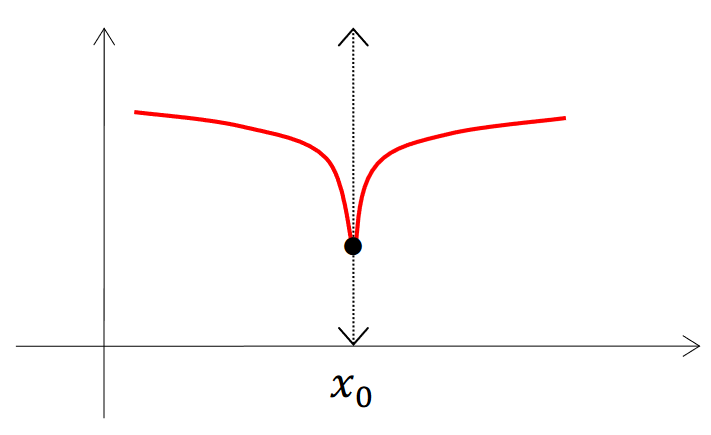
\includegraphics[width=0.4\textwidth]{cuspide.png}
\caption{Rappresentazione grafica di un punto di cuspide}
\end{figure}\\
Nel primo caso si dice che il punto è di cuspide con concavità verso l'alto, nel secondo caso si dice che il punto è di cuspide con concavità verso il basso.
\item \textbf{Punti di flesso a tangente verticale} Un punto $x_0$ è di flesso a tangente verticale se il limite destro e sinistro della derivata prima sono entrambi uguali a $+\infty$ oppure a $-\infty$\\
\[
    \lim_{x \to x_0^+} f'(x) =\lim _{x \to x_0^-} f'(x) = \pm \infty
\]
\begin{figure}[h]
    \centering
    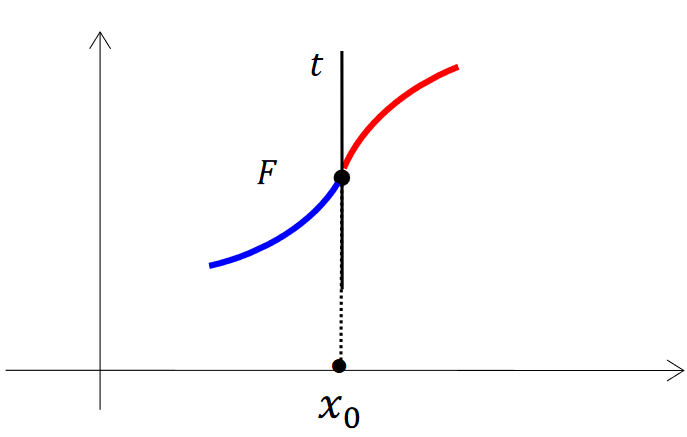
\includegraphics[width=0.4\textwidth]{flessotgv.png}
    \caption{Rappresentazione grafica di un punto di flesso a tangente verticale}
\end{figure}\\
\end{itemize}
\begin{esbox}
    %modulo di x%
    Sia $f(x)=|x|$.\\
    \begin{center}
        \begin{tikzpicture}
            \begin{axis}[
                    axis lines = center,
                    xlabel = $x$,
                    ylabel = {$f(x)$},
                    xmin=-5, xmax=5,
                    ymin=-5, ymax=5,
                    xtick={-5,-4,...,5},
                    ytick={-5,-4,...,5},
                ]
                \addplot [
                    domain=-5:5,
                    samples=100,
                    color=red,
                ]
                {abs(x)};
            \end{axis}
        \end{tikzpicture}
    \end{center}
    \begin{equation*}
        f'(x)=
        \begin{cases}
            1  & \text{se } x \geq 0 \\
            -1 & \text{se } x < 0
        \end{cases}
    \end{equation*}
    Rapporto incrementale per $x=0$
    \begin{equation*}
        \frac{f(x_0+h)-f(x_0)}{h}=\frac{|h|-|0|}{h}=\frac{|h|}{h}
    \end{equation*}
    $f'(|x|)=\frac{|x|}{x}$\\\\
    Il dominio di $f'(x)$ è $x \neq 0$\\
    Verifichiamo che tipo di punto è $x=0$\\
    \[
        \lim_{x \to 0^+} f'(x) = 1 \quad \land \quad \lim_{x \to 0^-} f'(x) = -1
    \]
    Quindi $x=0$ è un punto angoloso.
\end{esbox}
%punti stazionari%
\newpage
\section*{Punti stazionari}
Un punto stazionario è un punto in cui $f'(x)=0$.
I punti stazionari di una funzione sono i punti di massimo o minimo relativo.
\begin{itemize}
\item Se $f'(x_0)=0$ e $f''(x_0)>0$ allora $P(x_0,f(x_0))$ è un punto di minimo
relativo.
\begin{figure}[h]
    \centering
    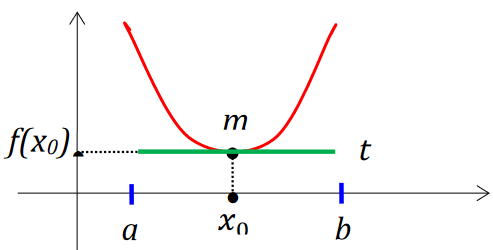
\includegraphics[width=0.4\textwidth]{minrel.png}
    \caption{Rappresentazione grafica di un punto di minimo relativo}
\end{figure}\\
\item Se $f'(x_0)=0$ e $f''(x_0)<0$ allora $P(x_0,f(x_0))$ è un punto di massimo
relativo.
\begin{figure}[h]
\centering
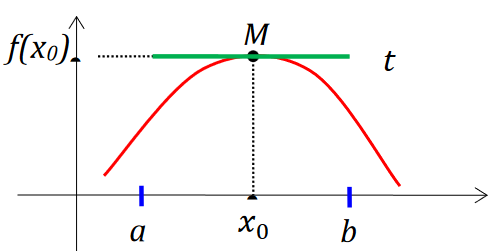
\includegraphics[width=0.4\textwidth]{maxrel.png}
\caption{Rappresentazione grafica di un punto di massimo relativo}
\end{figure}\\
\end{itemize}
\newpage
%Derivate delle funzioni elementari%
\textbf{Derivate delle funzioni elementari}
    \begin{itemize}
    \item $(c)'=0$
    \item $(x^n)'=nx^{n-1}$
    \item $(\sqrt{x})'=\frac{1}{2\sqrt{x}}$
    \item $(\frac{1}{x})'=-\frac{1}{x^2}$
    \item $(\sin x)'=\cos x$
    \item $(\cos x)'=-\sin x$
    \item $(\tan x)'=\frac{1}{\cos^2 x}$
    \item $(\arctan x)'=\frac{1}{1+x^2}$
    \item $(e^x)'=e^x$
    \item $(a^x)'=a^x\ln a$
    \item $(\log_a x)'=\frac{1}{x\ln a}$
    \item $(\ln x)'=\frac{1}{x}$
    \end{itemize}
\end{document}